\documentclass[journal,twoside,web]{ieeecolor}
\usepackage{tmi}
\usepackage{cite}
\usepackage{amsmath,amssymb,amsfonts}
\usepackage{algorithmic}
\usepackage{graphicx}
\usepackage{textcomp}

\usepackage{xcolor}

\makeatletter
\let\NAT@parse\undefined
\makeatother
\usepackage{hyperref}

\usepackage[capitalise,noabbrev]{cleveref}


\def\BibTeX{{\rm B\kern-.05em{\sc i\kern-.025em b}\kern-.08em
	T\kern-.1667em\lower.7ex\hbox{E}\kern-.125emX}}
\markboth{\journalname, VOL. XX, NO. XX, XXXX 2024}
{Tan \MakeLowercase{\textit{et al.}}: DeepDWI}


\newcommand{\argmin}{\operatornamewithlimits{argmin}}
\newcommand{\norm}[1]{\left\lVert#1\right\rVert}


\begin{document}
	\title{Diffusion-Weighted Imaging with Learned Nonlinear Latent Space Modeling and Self-Supervised Reconstruction (DeepDWI)}

	\author{Zhengguo Tan, Julius Glaser, Patrick A Liebig, Annika Hofmann, Frederik B Laun, Florian Knoll
		\thanks{This work was supported in part by
			German Research Foundation (DFG)
			under projects 513220538 and 512819079,
			project 500888779 in the Research Unit RU5534
			for MR biosignatures at UHF,
			and by the National Institutes of Health (NIH)
			under grants R01 EB024532 and P41 EB017183.
			In addition, scientific support and HPC resources
			were provided by
			the Erlangen National High Performance Computing Center (NHR)
			of Friedrich-Alexander-University Erlangen-Nuremberg (FAU)
			under the NHR project b143dc.
			NHR is funded by federal and Bavarian state authorities.
			NHR@FAU hardware is partially funded by
			DFG under project 440719683.}
		\thanks{Z.~Tan was with the Department
			Artificial Intelligence in Biomedical Engineering (AIBE),
			FAU, Erlangen, Germany.
			He is now with
			the Michigan Institute for Imaging Technology and Translation
			(MIITT),
			Department of Radiology,
			University of Michigan, Ann Arbor, MI 48109 USA
			(e-mail: zgtan@med.umich.edu).}
		\thanks{J.~Glaser was with the Department of Medical Engineering,
			FAU, Erlangen, Germany.
			He is now with the Institute of Radiology,
			University Hospital Erlangen,
			FAU, Erlangen, Germany
			(e-mail: julius.glaser@fau.de).}
		\thanks{P.~A.~Liebig is with Siemens Healthcare GmbH, Erlangen, Germany
			(e-mail: patrick.liebig@siemens-healthineers.com).}
		\thanks{A.~Hofmann is with the Department AIBE,
			FAU, Erlangen, Germany
			(e-mail: annika.ah.hofmann@fau.de).}
		\thanks{F.~B.~Laun is with the Institute of Radiology,
			University Hospital Erlangen,
			FAU, Erlangen, Germany
			(e-mail: Frederik.Laun@uk-erlangen.de).}
		\thanks{F.~Knoll is with the Department AIBE,
			FAU, Erlangen, Germany
			(e-mail: florian.knoll@fau.de).}
	}

	\maketitle

	% Keep the abstract to 250 words or less.
	\begin{abstract}
		% Define all symbols used in the abstract. Do not cite references in the abstract.
		The code is publicly available at: \url{https://github.com/ZhengguoTan/DeepDWI}.
	\end{abstract}

	\begin{IEEEkeywords}
	Diffusion-weighted imaging, Image reconstruction, Generative AI, Latent space, Self-supervised learning
	\end{IEEEkeywords}

	% ============================== %
	\section{Introduction}
	\label{SEC:INTRO}
	\IEEEPARstart{H}{igh}-dimensional magnetic resonance imaging (HD-MRI)
	has been an emerging and flourishing field,
	which has achieved substantial improvements in terms of spatiotemporal fidelity.
	Instead of the conventional two-dimensional static single-contrast-weighted imaging,
	HD-MRI acquires and reconstructs multi-dimensional information.
	For instance, Brown et al.~\cite{brown_1982_mrsi}
	proposed magnetic resonance spectroscopic imaging (MRSI),
	which uses multiple readout gradients to acquire multiple echo images
	for the computation of spatially resolved metabolic distribution.
	Le BiHan et al.~\cite{lebihan_1986_diff} and
	Merboldt et al.~\cite{merboldt_1985_diff} proposed
	diffusion-weighted imaging (DWI),
	which utilizes spatially and angularly varying
	diffusion encoding gradients in combination with
	fast echo-planar imaging (EPI) readouts \cite{mansfield_1977_epi}
	to obtain multi-contrast diffusion-weighted images
	as a probe into tissue microstructure.
	Ma et al.~\cite{ma_2013_mrf} proposed
	magnetic resonance fingerprinting (MRF)
	which consists of a $T_1$- and $T_2$-prepared pseudo-randomized sequence
	to acquire time-resolved transient-state images
	and a Bloch-equation-based dictionary matching algorithm \cite{doneva_2010_moba}
	for simultaneous quantitative $T_1$ and $T_2$ mapping.

	HD-MRI, however, conventionally requires long scan time.
	Advances in parallel imaging
	\cite{roemer_1990_pi,sodickson_1997_smash,
	pruessmann_1999_sense,pruessmann_2001_gsense,griswold_2002_grappa}
	and compressed sensing
	\cite{lustig_2007_cs,block_2007_cs,liang_2007_psf}
	have enabled accelerated acquisition for HD-MRI.
	In particular, the low-rank modeling and regularization \cite{cai_2010_svt}
	has been a powerful tool in reducing the dimensionality of high-dimensional data,
	which enables accelerated acquisition and high spatiotemporal-resolution reconstruction.
	Usually, singular value decomposition (SVD) is used to
	learn a truncated temporal basis function from
	a large-scale physics-informed dictionary
	\cite{huang_2012_t2basis,lam_2014_spice,mcgivney_2014_svdmrf}.
	The temporal basis function is then integrated
	with the MRI forward model,
	i.e.~the sensitivity encoding operator \cite{pruessmann_2001_gsense},
	for joint reconstruction of the corresponding spatial basis images.
	In addition, low-rank regularization can be employed in the joint reconstruction
	\cite{tamir_2017_t2shuffling}.

	Beyond the low-rank technique,
	advanced neural networks, e.g.~autoencoder \cite{hinton_2006_ae},
	have been explored for HD-MRI reconstruction and
	proven to supply more accurate representations of
	high-dimensional data than SVD.
	Lam et al.~\cite{lam_2019_mrsi} and Mani et al.~\cite{mani_2021_qmodel}
	proposed to first learn a denoising autoencoder (DAE) model
	from a physics-informed simulated dictionary
	and then incorporate the learned DAE model as a regularizer
	in the alternating direction method of multipliers (ADMM)
	\cite{boyd_2010_admm}
	unrolling reconstruction.
	Pioneered by Gregor and LeCun \cite{gregor_2010_algunroll},
	algorithm unrolling enables the use of learned deep \textit{prior}
	as regularization and faster inference than
	iterative reconstruction with hand-crafted regularization functions
	\cite{monga_2021_algunroll}.
	Algorithm unrolling has been introduced to
	accelerated MRI reconstruction and
	employed in various scenarios:
	supervised learning with fully sampled reference images
	\cite{hammernik_2018_varnet,aggarwal_2018_modl},
	self-supervised learning
	with only undersampled data available for training
	\cite{yaman_2020_ssdu,yaman_2022_zs}.

	Deep neural networks are capable of learning
	not only regularization functions,
	but also MR-physics forward operators.
	Zhu et al.~\cite{zhu_2018_automap} proposed
	the automated transform by manifold approximation (AUTOMAP),
	which learns the mapping between the sensor and the image domain
	for data-driven supervised image reconstruction.
	Liu et al.~\cite{liu_2021_relax} proposed
	the reference-free $T_1$ parameter maps extraction (RELAX)
	self-supervised deep learning reconstruction,
	which learns the mapping from $T_1$ parameter maps to
	undersampled multi-coil multi-contrast $k$-space data.
	Arefeen et al.~\cite{arefeen_2023_latent} proposed
	to replace the conventional SVD-based linear subspace modeling
	\cite{huang_2012_t2basis}
	by the latent decoder model within DAE
	for improved $T_2$-weighted image reconstruction.

	Several challenges exist when adopting deep learning to
	DWI reconstruction.
	First, the capability of DAE to learn diffusion MRI models
	is open to questions.
	DAE is composed of sequential fully connected layers
	with nonlinear activation functions.
	This simple architecture may fail to learn complicated functions.
	DWI signal is such an example.
	The standard diffusion tensor model \cite{basser_1994_dmri}
	consists of six tensor elements,
	and forms DWI signals based on
	the multiplication of exponential functions.
	Second, it is rather difficult to acquire fully-sampled data
	for the training of a regularization functional.
	On the one side,
	fully sampled DWI requires a longer echo train in EPI,
	which not only elongates the scan time
	but also increases off-resonance-induced geometric distortion.
	On the other side,
	there exists a wide range of diffusion acquisition modes,
	thereby requiring a larger dataset than
	the two-dimensional imaging scenario.
	% Moreover, DWI signals can be described with more complicated models,
	% e.g.~the ball-and-stick model \cite{behrens_2003_ballstick},
	% which involves even more parameters.

	To overcome these challenges,
	we aim to develop a generalized DWI reconstruction framework
	with learned nonlinear latent space modeling and
	self-supervised reconstruction,
	dubbed DeepDWI.


	% ============================== %
	\section{Related Work}

	\begin{figure*}
		\centering
		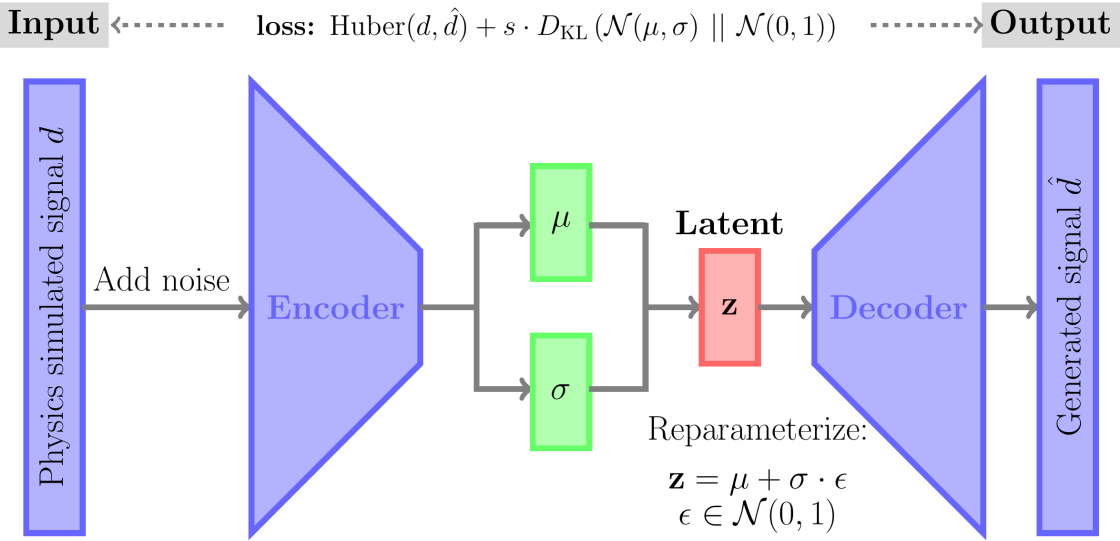
\includegraphics[width=\textwidth]{../figures/fig1.png}
		\caption{\textbf{(A)} The architecture of a variational autoencoder.
			\textbf{(B)} An illustration of the joint $k$-$q$-slice forward operator
			for multi-band multi-shot DWI acquisition.
			$[x, y, z, q]$ denotes the shape of input DWI ($\mathbf{\tilde{x}}$),
			with $x$ and $y$ as the image size, $z$ as the number of slices,
			and $q$ as the number of diffusion encodings.
			The operator outputs multi-dimensional $k$-space with the shape $[x, y, 1, c, q, s]$,
			with $c$ as the number of receiver coils, $s$ as the number of shots.}
		\label{FIG:MODEL}
	\end{figure*}

	\subsection{Variational Autoencoder (VAE)}

	Autoencoders (AEs) are neural network type trained in an unsupervised manner. 
	They utilize two smaller networks an encoder and a decoder, connected through a latent space. 
	The trained encoder acts as a dimensionality reducer, producing a compact sparse representation of the data in the latent space.
	The decoder is trained to reconstruction the input data from the encoder produced latent representation. 
	Because the the standard AE training scheme does not constrain the latent space in any way, the network has problems to generalize.
	The Variational Autoencoder (VAE) was first introduced by Kingma and Welling \cite{kingma_2014_vae} and uses the principle of variational inference. 
	By that the VAE is forced to learn the probability distributions of the latent variables and a second term is 
	added to the loss function of the network, the result of the Kullbeck Leibler Divergence, which describes how much the 
	learned latent distributions diverge from the real distributions by that regularizing the reconstruction training. 
	The latent space in VAE is not consisting of simple neurons but 
	resambles distributions of the latent activations and samples from these. 
	The sampling operation is not backpropagateable, however, 
	so the network makes use of the reparameterization trick - 
	the VAE learns a mean and a variance for each latent variable 
	and these are used to scale the drawn samples from a gaussian distribution (mean=0, variance=1).
	In \cref{FIG:MODEL} (A) the used VAE model is shown.

	\subsection{Multi-Band Multi-Shot DWI Acquisition \& Modeling}

	\cref{FIG:MODEL} (B) illustrates the joint $k$-$q$-slice forward forward operator
	for multi-band multi-shot DWI acquisition \cite{tan_2024_naviepi}.
	This operator can be understood as
	an extended sensitivity encoding (SENSE) operator \cite{pruessmann_2001_gsense},
	which maps the multi-slice multi-diffusion-weighted images ($\mathbf{\tilde{x}}$)
	to their corresponding $k$-space,
	\begin{equation}
		\mathcal{A}(\mathbf{\tilde{x}}) = \mathbf{P \Sigma \Theta F S \Phi} \mathbf{\tilde{x}}
		\label{EQU:FWD}
	\end{equation}
	Here, the images $\mathbf{\tilde{x}}$ are point-wise multiplied
	with the pre-computed shot-to-shot phase variation maps ($\mathbf{\Phi}$)
	and coil sensitivity maps ($\mathbf{S}$).
	The output images are then converted to $k$-space
	via two-dimensional fast Fourier transform ($\mathbf{F}$),
	point-wise multiplied with the multi-band phases ($\mathbf{\Theta}$),
	summed along the slice dimension ($\mathbf{\Sigma}$),
	and then multiplied by the undersampling mask ($\mathbf{P}$).

	With the operator $\mathcal{A}$, the inverse problem in DWI reads,
	\begin{equation}
		\argmin_{\mathbf{\tilde{x}}} \norm{\mathbf{y} - \mathcal{A}(\mathbf{\tilde{x}})}_2^2 + \lambda \mathcal{R}(\mathbf{\tilde{x}})
		\label{EQU:INV}
	\end{equation}
	where $\mathbf{y}$ is the measured $k$-space data.
    The first term in \cref{EQU:INV} presents data consistency, and
    the second term presents the regularization function $\mathcal{R}(\tilde{x})$
	with the regularization strength $\lambda$.
	When using the Tikhonov regularization,
	i.e.~$\mathcal{R}(\mathbf{\tilde{x}}) = \norm{\mathbf{\tilde{x}}}_2^2$,
	\cref{EQU:INV} can be solved via the conjugate gradient (CG) method.


	\subsection{Algorithm Unrolling for Image Reconstruction}

    % Algorithm unrolling has been an emerging technique
    % in solving \cref{EQU:INV}, which consists of two ingredients.
    % First, algorithm unrolling learns a regularization function
    % via deep neural networks.
    % Second, algorithm unrolling is constrained
    % by the data-consistency term,
    % i.e., the forward pass of the estimate $\mathcal{A} (\mathbf{\tilde{x}})$
    % must be close to the measured data $\mathbf{y}$.

    Similar to conventional optimization algorithms,
    algorithm unrolling requires iterative procedures
    to solve \cref{EQU:INV}. In MRI image reconstruction,
    two algorithm unrolling approaches have been proposed.
    The first one is known as the variational network (VarNet)
    \cite{hammernik_2018_varnet}, whose update rule reads
    \begin{equation} \label{EQU:VarNet_Upd}
        \left\{\begin{aligned}
            \mathbf{z}^{(k)} &= \mathbf{\tilde{x}}^{(k)} - \lambda \cdot \mathcal{A}^H \Big( \mathcal{A} (\mathbf{\tilde{x}}^{(k)}) - \mathbf{y} \Big) \\
            \mathbf{\tilde{x}}^{(k+1)} &= \mathbf{z}^{(k)} - \mathcal{N}_{\theta}^{(k)} (\mathbf{z}^{(k)})
        \end{aligned}\right.
    \end{equation}
    with $k$ being the iteration step.
    To learn the parameters $\theta$ and the gradient step size $\lambda$,
    the loss function in VarNet is given as
    \begin{equation}
        \argmin_{(\theta^{(1)}, \ldots, \theta^{(K)}, \lambda)} \mathcal{L} (\mathbf{x}_{\text{ref}}, \mathbf{\tilde{x}}^{(K)}) = \norm{\mathbf{\tilde{x}}^{(K)} - \mathbf{x}_{\text{ref}}}_2^2
        \label{EQU:VarNet_Loss}
    \end{equation}
    where $\mathbf{\tilde{x}}^{(K)}$ is the estimate after $K$ iterations,
    and $\mathbf{x}_{\text{ref}}$ denotes fully-sampled reference images.
    Here, the neural network parameters $\theta$
    differ among iterations.

    The second algorithm unrolling in MRI is known as
    Model-based deep learning architecture for inverse problems (MoDL)
    \cite{aggarwal_2018_modl},
    which tends to learn a denoising neural network,
    and redefines \cref{EQU:INV} as
    \begin{equation}
		\argmin_{\mathbf{\tilde{x}}} \norm{\mathbf{y} - \mathcal{A}(\mathbf{\tilde{x}})}_2^2 + \lambda \norm{ \mathbf{\tilde{x}} - \mathcal{D}_{\omega}(\mathbf{\tilde{x}}) }_2^2
		\label{EQU:DINV}
	\end{equation}
    Instead of the VarNet update rule in \cref{EQU:VarNet_Upd},
    MoDL employs the alternating minimization scheme,
    \begin{equation} \label{EQU:MoDL_Upd}
        \left\{\begin{aligned}
            \mathbf{z}^{(k)} &= \mathcal{D}_{\omega} (\mathbf{\tilde{x}}^{(k)}) \\
            \mathbf{\tilde{x}}^{(k+1)} &= \argmin_{\mathbf{x}} \norm{\mathbf{y} - \mathcal{A}(\mathbf{x})}_2^2 + \lambda \norm{ \mathbf{x} - \mathbf{z}^{(k)} }_2^2
        \end{aligned}\right.
    \end{equation}
    where the second minimization problem is solved by CG.
    MoDL shares weights among iterations, and thus the loss function reduces to
    only one set of model parameters.
    Both VarNet and MoDL require reference images,
    and thus fall into the category of supervised learning.

    In practice, it is challenging to acquire fully-sampled reference images.
    To enable deep neural network training without fully sampled reference data,
    Yaman et al.~\cite{yaman_2020_ssdu} proposed self-supervised learning via data undersampling (SSDU).
    In SSDU, the undersampled data is partitioned into two disjoint sets,
    one for the data-consistency term, and another for the loss function calculation.
    Thus, the sampling mask $\mathbf{P}$ splits,
    \begin{equation}
        \mathbf{P} = \Theta ~\cup~ \Lambda
    \end{equation}
    SSDU follows the alternating update scheme in MoDL,
    and such a splitting leads to two modifications in training.
    First, the $k$-space data and the forward model in \cref{EQU:MoDL_Upd} is masked as
    $\mathbf{y}_{\Theta}$ and $\mathcal{A}_{\Theta}$, respectively.
    Second, the loss function is computed in $k$-space,
    \begin{equation}
        \argmin_{(\theta, \lambda)} \mathcal{L} (\mathbf{y}_{\Lambda}, \mathcal{A}_{\Lambda}(\mathbf{\tilde{x}}^{(K)}))
        \label{EQU:SSDU_Loss}
    \end{equation}
    where a normalized $\ell_1$-$\ell_2$ loss is used \cite{yaman_2020_ssdu}.
    Further, Yaman et al.~\cite{yaman_2022_zs} proposed subject-specific zero-shot learning,
    where one single scan data is partitioned into three disjoint sets,
    two used to enforce data consistency and to update loss,
    and the last served as self-validation to allow for early stopping.

	% The regularization function in \cref{EQU:INV} can be nonlinear,
	% e.g.~the sparsity \cite{lustig_2007_cs} or the low-rankness \cite{liang_2007_psf} constraint.
	% In this scenario, algorithms such as
	% the fast iterative shrinkage thresholding (FISTA) \cite{beck_2009_fista}
	% and the alternating direction method of multipliers (ADMM) \cite{boyd_2010_admm}
	% are often employed.
	% These algorithms consist of a substep that transforms $\mathbf{\tilde{x}}$
	% to a sparsifying domain or a specialized matrix format
	% (e.g., the spatial-diffusion matrix in our previous work \cite{tan_2024_naviepi})
	% and then performs nonlinear thresholding to promote sparsity or low-rankness.
	% This substep shares similarities to deep neural networks,
	% and inspires the seminal work on algorithm unrolling
	% by Gregor and LeCun \cite{gregor_2010_algunroll}.
	% Instead of a hand-crafted regularization function,
	% algorithm unrolling learns deep \textit{prior}
	% via the use of deep neural networks as the regularization function.
	% This enables the learning of true image \textit{prior} during the training process
	% and much faster inference than iterative reconstruction with hand-crafted regularization functions.
	% An excellent review of algorithm unrolling
	% has been provided by Monga et al.~\cite{monga_2021_algunroll}.

	% In the area of image reconstruction for accelerated MRI,


	% ============================== %
	\section{Methods}



	% ============================== %
	\section{Results}

	\subsection{VAE enables robust \& accurate learning of DWI signal}

	\subsection{Zero-shot learning enables motion-robust DWI}

	\subsection{Zero-shot learning: model generalization}

	\subsection{VAE modeling with zero-shot learning reconstruction}


	% ============================== %
	\section{Discussion}


	% ============================== %
	\section{Conclusion}


	% ============================== %
	\section*{Acknowledgment}

	Z.~Tan thanks to Ms.~Soundarya Soundarresan for
	her work and discussion on denoising autoencoder,
	and to Dr.~Xiaoqing Wang for
	the discussion on self-supervised learning.

	% ============================== %
	\bibliographystyle{IEEEtran}
	\bibliography{../../ref/ref}

\end{document}
